\section{A Ground Motion Prediction Equation (GMPE) Toolkit}
\label{sec:gmpe_toolkit}

Probabilistic Seismic Hazard Assessment (PSHA) is well-established as a robust and effective means of characterising the level of ground shaking to which a structure may be subject within a given time period. Since its inception in the 1960s the PSHA methodology undergone many developments designed to improve the characterisation of the physical properties of the rupture source, the ground motion attenuation and the site amplification. Often leading these developments are the Ground Motion Prediction Equations (GMPEs), which characterise the manner in which ground motion measures (intensity measures) vary with the source, path and site properties of observed ground motion records. 

The widespread adoption of PSHA for site-specific, urban-level and national/regional-scale analyses of earthquake hazard has created a clear need for calculation software to be widely available for this purpose. Furthermore, in recent years that has been an increasing need for PSHA calculation software to be widely available, for its processes to be open, and for a commitment to quality assurance. Recognising this need the Global Earthquake Model (GEM) Foundation created OpenQuake, an open-source software for calculation of probabilistic seismic hazard and risk, that is developed using a test-driven philosophy in which the software undergoes extensive testing and quality assurance as part of the construction process. 

Whilst OpenQuake itself is designed to fullfill the need for open and tested software for PSHA calculation, it does not explicitly address the issue of PSHA model construction. A PSHA model can be broken down into three components: the seismogenic source model(s), the ground motion prediction equations and the logic tree to characterise the model-to-model uncertainty in an equation. GEM is now in the process of endeavouring to extend the OpenQuake development approach to the area of PSHA model construction. It has done so with the development of two ``Modeller's Toolkit's: 

\begin{enumerate}
\item \textbf{The Hazard Modeller's Toolkit} , a suite of open-source tools for the preparation of seismogenic source models for application in PSHA \cite{hmtk_guide}
\item \textbf{The OpenQuake Ground Motion Toolkit}, a suite of open-source tools for analysis and interpretation of observed ground motions and ground motion prediction equations, for the purposes of GMPE selection in PSHA (this document)
\end{enumerate}

This document presents the OpenQuake Ground Motion Toolkit, or GMPE-SMTK hereafter, providing an overview of the features as well as practical examples that demonstrate how to use the toolkit in real applications. 

\section{Objectives and Structure}
\label{sec:objectives}

The GMPE-SMTK serves the primary objective of assisting seismic hazard modellers with the process of understanding and identifying GMPEs for application in seismic hazard analysis. It brings together a collection of tools for visualising and exploring ground motion prediction equations, for analysing ground motion records to derive widely used ground motion intensity measures, and to compare observed ground motion intensity levels against the values predicted by the GMPE. To do this, however, the GMPE-SMTK has needed to create an internal data structure to store and process databases of ground motion records. A general overview of the GMPE-SMTK is shown in Figure \ref{fig:smtk_overview}.

\begin{figure}[htb]
	\centering
		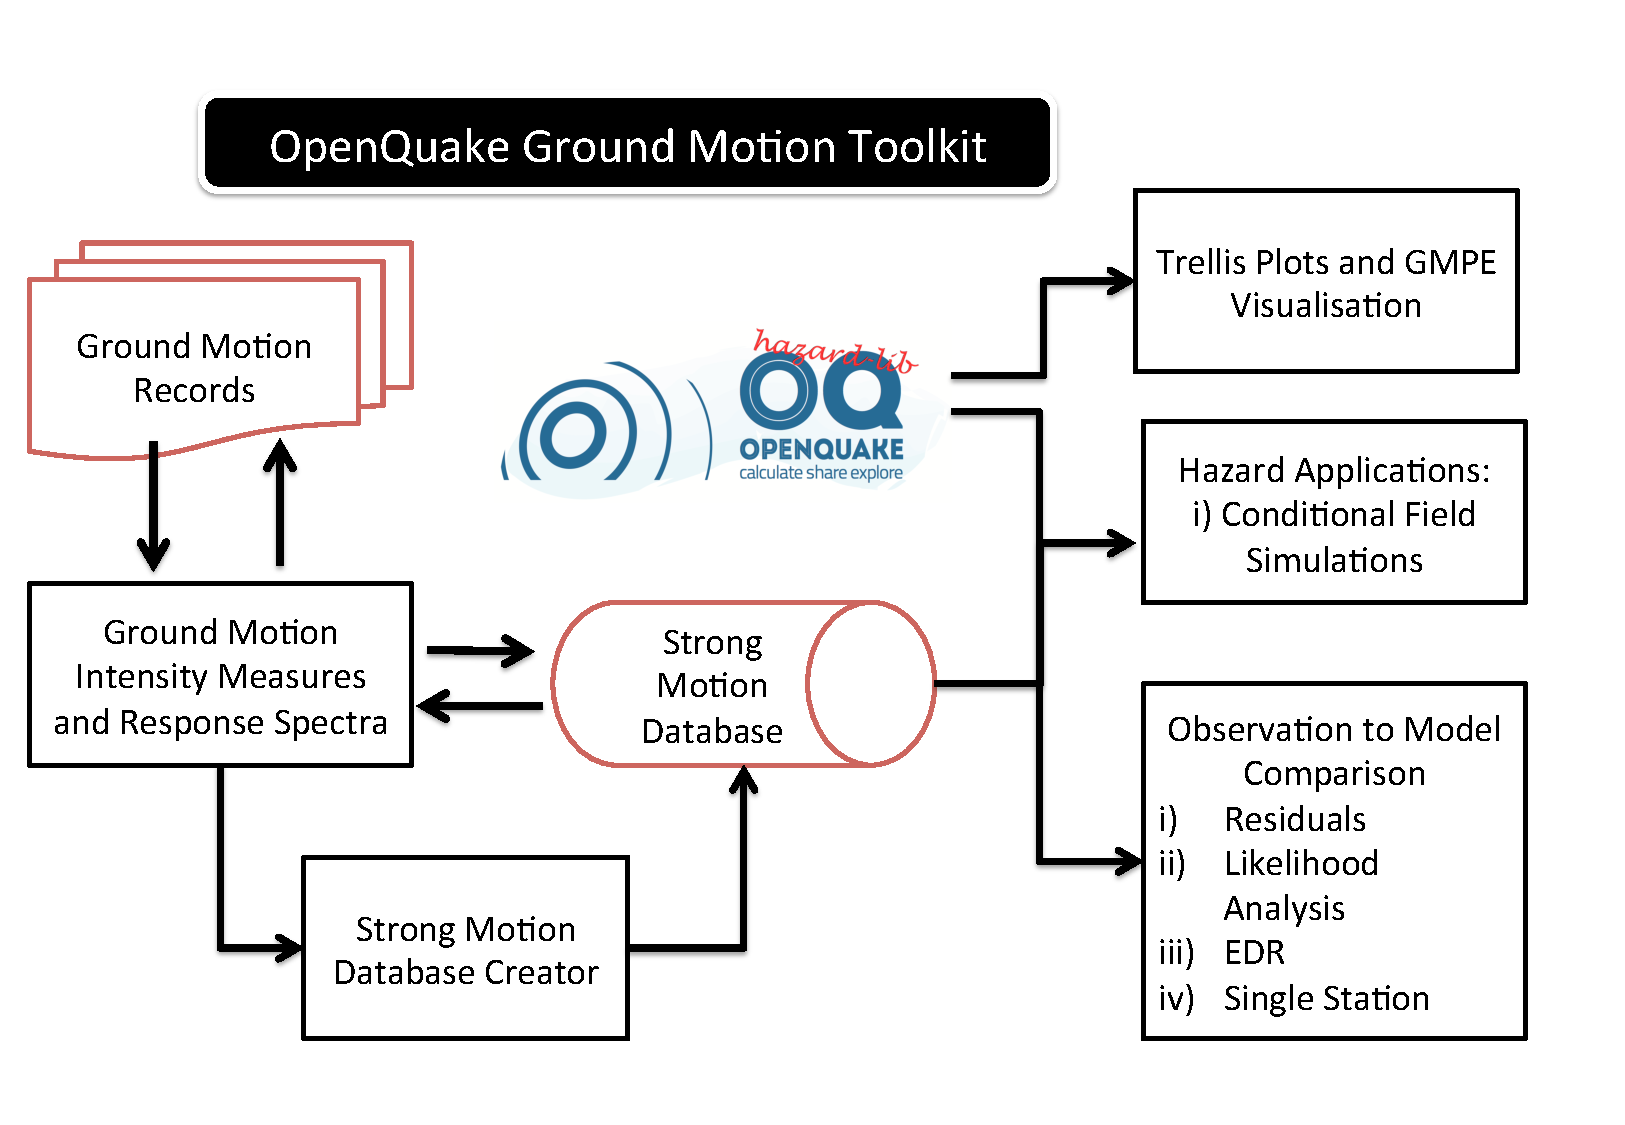
\includegraphics[width=\textwidth]{./figures/intro/smtk_architecture_flowchart.pdf}
	\caption{Feature Overview of the OpenQuake Ground Motion Toolkit}
	\label{fig:smtk_overview}
\end{figure}

The critical element within this process is the usage of OpenQuake, or more specifically the OpenQuake Hazard Library, as a dependency within the toolkit. It is from this library that we take the GMPEs, as well as various tools for undertaking calculations of source to site geometry. By using OpenQuake's own library we inherit OpenQuake's testing and quality assurance process for implementation of GMPEs. We also ensure total consistency between the GMPEs used for comparison against strong motion records and those used within the OpenQuake PSHA calculation engine itself. This is a feature that is unique to this toolkit. 

A list of the current functionalities is given in Table \ref{tab:features}.

\begin{table}
\centering
\begin{tabular}{|c|c|} \hline
\textbf{Feature} & \textbf{Algorithm} \\ \hline
Ground Motion  &  Retrieve PGA, PGV and PGD \\
Intensity Measures  &  Response Spectra - Newmark-$\beta$ \\
  &   Response Spectra - \cite{NigamJennings1969} \\
  &   Horizontal Spectra (Geometric Mean, Envelope etc.) \\
  &   Rotate Horizontal Record Pairs \\
  &   Rotational Spectra (GMRotD, GMRotI) \cite{Boore_etal2006} \\ \hline
Trellis Plotting & Configure Rupture \\
                 & Compare GMPE Scaling with Magnitude \\
                 & Compare GMPE Scaling with Distance \\
                 & Compare GMPE Spectra with Magnitude \& Distance \\ \hline
Comparison with  & Get GMPE residuals from Ground Motion ... \\
Observations     & ... measure residual distribution \\
                 & ... retrieve inter- and intra-event residual \\
                 & ... view trends with magnitude \\
                 & ... view trends with distance \\
                 & ... view trends with $V_{S30}$ \\
                 & ... view trends with event depth \\
                 & Likelihood Analysis \cite{Scherbaum_etal2004}\\
                 & Log-likeihood Analysis \cite{Scherbaum_etal2009}\\
                 & Euclidean Distance-Based Ranking \cite{KaleAkkar2013}\\
                 & Single-Site Residual Analysis \\ \hline
Hazard Applications & Conditional Field Simulation \\ \hline
\end{tabular}
\caption{Current features within the OpenQuake Ground Motion Toolkit}
\label{tab:features}

\end{table}

\section{Installation and Getting Started}
\label{sec:installation}

The software is available on the open Github repository: \href{https://github.com/g-weatherill/gmpe-smtk}{https://github.com/g-weatherill/gmpe-smtk}. Installation is dependent on the OpenQuake hazardlib and nrmllib libraries. These can be retrieve from the following repositories:
\begin{itemize}
\item OpenQuake Hazard Library (oq-hazardlib)\\
\href{https://github.com/gem/oq-hazardlib}{https://github.com/gem/oq-hazardlib}
\item OpenQuake Natural Risk Markup Language (NRML) Library (oq-nrmllib)\\
\href{https://github.com/gem/oq-nrmllib}{https://github.com/gem/oq-nrmllib}
\end{itemize}

The GMPE-SMTK has the following dependencies:

\begin{itemize}
\item \textbf{Numpy 1.6.1 or later}
\item \textbf{Scipy 0.11.0 or later}
\item \textbf{Matplotlib 1.3.x or later}
\item \textbf{H5py 2.2.0 or later}
\item \textbf{lxml}
\item \textbf{Shapely 1.2.18 or later}
\item \textbf{oq-hazardlib (brings in Numpy, Scipy and Shapely)}
\item \textbf{oq-nrmllib (brings in lxml\footnote{Except on Windows})} 
\end{itemize}


\subsection{Windows}

For a comprehensive Python installation including many of the dependencies needed to both the toolkit and the OpenQuake libraries the best option is a full installation of PythonXY. This software is freely available from here: \href{https://code.google.com/p/pythonxy/}{https://code.google.com/p/pythonxy/}. It is recommended to proceed with a \emph{full} installation and ensure that all of the above dependencies are selected for installation where available.

For the oq-nrmllib it is necessary to install the Lxml library (\href{http://lxml.de}{http://lxml.de}). This is not officially supported for Windows, so it is recommended (by Python developers themselves!) to install the unofficial Lxml binding from here: \footnote{\href{http://www.lfd.uci.edu/~gohlke/pythonlibs/}{http://www.lfd.uci.edu/~gohlke/pythonlibs/}}. Download and then run the 32-bit package named ``lxml-\#.\#.\#.win32-py2.7.exe''.

Next you will need to install the op-hazardlib and oq-nrmllib. From the web repositories listed previously click the button ``Download Zip'', then extract contents to the folders \verb=C:/oq-hazardlib= and \verb=C:/oq-nrmllib= respectively.

Open an enhanced IPython console. Go to Start $->$ Python(xy) $->$ Enhanced Consoles $->$ Ipython (sh). This will open up an Ipython console terminal. To install the oq-hazardlib, at the console prompt type:

\begin{Verbatim}[frame=single, commandchars=\\\{\}, fontsize=\scriptsize]
~$: cd C:/oq-hazardlib/
~$: python setup.py install build --compiler=mingw32
\end{Verbatim}

This will install the oq-hazardlib with the full C-extensions, which speed up some of the geometry calculations. Then do the same with the oq-nrmllib.

\begin{Verbatim}[frame=single, commandchars=\\\{\}, fontsize=\scriptsize]
~$: cd C:/oq-hazardlib/
~$: python setup.py install
\end{Verbatim}

Then close the console by typing \verb=exit=. 

Finally, download the zipped folder of the GMPE-SMTK from the github repository and unzip to a folder of your choosing. To allow for usage of the GMPE-SMTK throughout your operating system, do the following: 

\begin{enumerate}
\item From the desktop, right-click \textbf{My Computer} and open \textbf{Properties}
\item In the ``System Properties'' window click on the \textbf{Advanced} tab.
\item From the ``Advanced'' section open the \textbf{Environment Variables}.
\item In the ``Environment Variables'' you sill see a list of ``System Variables'', select ``Path'' and ``Edit''.
\item Add the path to the hmtk directory to the list of folders then save.
\end{enumerate}

After this process it may be necessary to restart PythonXY.

\subsection{OSX and Linux}

For installation on unix platforms we recommend installing each package using the Python Package manager (Pip). Assuming that Python 2.7.3 is already installed on your system, the Package Manager can be installed using the command line:

\begin{verbatim}
~$ python get-pip.py 
\end{verbatim}

First it is recommended to install the OpenQuake libraries (as they bring in most of the dependencies!). These can be done using Git to clone the repositories:

\begin{verbatim}
# Clone the hazardlib repository
git clone https://github.com/gem/oq-hazardlib.git
cd oq-hazardlib
# Run the installation
sudo python setup.py install
cd ..
# Clone the nrmllib repository
git clone https://github.com/gem/oq-nrmllib.git
cd oq-nrmllib
sudo python setup.py install
\end{verbatim}

Then use PiP to install Matplotlib and H5py:

\begin{verbatim}
# Install Matplotlib
sudo pip install matplotlib
# Install H5py
sudo pip install h5py
\end{verbatim}

Finally all that is needed is to install the GMPE-SMTK. As with the OpenQuake libraries the best option is to use Git to clone the repository:

\begin{verbatim}
# Clone the repository
~$ git clone https://github.com/g-weatherill/gmpe-smtk.git
\end{verbatim}

As the repository does not have an installer the directory should be added manually to the Pythonpath. This can be done from the bash profile script using a suitable text editor (Vim in the example below):

\begin{verbatim}
# Open the profile script
~$ vim ~/.profile
# Add the following line to the bottom of the profile script
export PYTHONPATH=/Users/GW/Documents/GEM/hmtk/gmpe-smtk/:$PYTHONPATH
# Save and exit
\end{verbatim}

To complete the installation simply re-start the terminal.








